\documentclass[tikz,border=5pt]{standalone}
\usepackage{pgfplots}
\usetikzlibrary{shapes.geometric, intersections, calc}
\pgfplotsset{compat=1.7}

\begin{document}
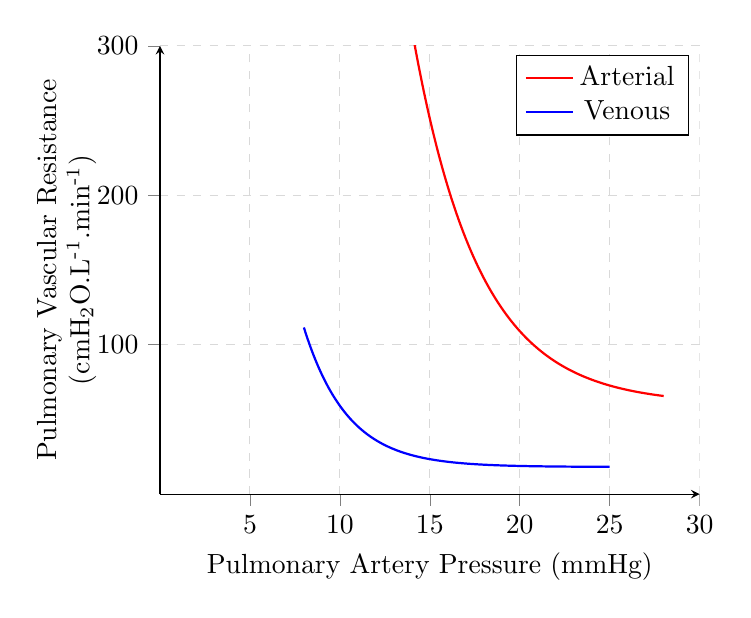
\begin{tikzpicture}
    \begin{axis}[
        axis x line=middle,
        axis y line=middle,
        grid = major,
        grid style={dashed, gray!30},
    	  x label style={at={(axis description cs:0.5,-0.1)},anchor=north},
	  y label style={at={(axis description cs:-0.1,.5)},rotate=90,anchor=south,align=center},
        xmin=0,
        xmax= 30,
        ymin= 0,
        ymax= 300,
	xlabel near ticks,
        xlabel=Pulmonary Artery Pressure (mmHg),
        ylabel=Pulmonary Vascular Resistance \\ (cmH\textsubscript{2}O.L\textsuperscript{-1}.min\textsuperscript{-1}),
        tick align=outside,
        enlargelimits=false]
	\coordinate (o) (0,0);

	\addplot[domain=12:28, red, thick,samples=500] {60.12674 + 11374.62*e^(-0.2724082*x)};
\addlegendentry{Arterial};

	\addplot[domain=8:25, blue, thick,samples=500] {18.18643 + 2518.857*e^(-0.411953*x)};
\addlegendentry{Venous};


\end{axis}


\end{tikzpicture} 
\end{document}